\documentclass[aspectratio=169]{beamer}
\usepackage{ferres}
\usepackage{tikz}
\usepackage{algorithm}
\usepackage[noend]{algpseudocode}
\usepackage{capt-of}
\usepackage{subcaption}
%math
\setbeamercolor{alerted text}{fg=red,bg=white}
%%%%% NEW MATH DEFINITIONS %%%%%

\usepackage{amsmath,amsfonts,bm}

% Mark sections of captions for referring to divisions of figures
\newcommand{\figleft}{{\em (Left)}}
\newcommand{\figcenter}{{\em (Center)}}
\newcommand{\figright}{{\em (Right)}}
\newcommand{\figtop}{{\em (Top)}}
\newcommand{\figbottom}{{\em (Bottom)}}
\newcommand{\captiona}{{\em (a)}}
\newcommand{\captionb}{{\em (b)}}
\newcommand{\captionc}{{\em (c)}}
\newcommand{\captiond}{{\em (d)}}

% Highlight a newly defined term
\newcommand{\newterm}[1]{{\bf #1}}


% Figure reference, lower-case.
\def\figref#1{figure~\ref{#1}}
% Figure reference, capital. For start of sentence
\def\Figref#1{Figure~\ref{#1}}
\def\twofigref#1#2{figures \ref{#1} and \ref{#2}}
\def\quadfigref#1#2#3#4{figures \ref{#1}, \ref{#2}, \ref{#3} and \ref{#4}}
% Section reference, lower-case.
\def\secref#1{section~\ref{#1}}
% Section reference, capital.
\def\Secref#1{Section~\ref{#1}}
% Reference to two sections.
\def\twosecrefs#1#2{sections \ref{#1} and \ref{#2}}
% Reference to three sections.
\def\secrefs#1#2#3{sections \ref{#1}, \ref{#2} and \ref{#3}}
% Reference to an equation, lower-case.
\def\eqref#1{equation~\ref{#1}}
% Reference to an equation, upper case
\def\Eqref#1{Equation~\ref{#1}}
% A raw reference to an equation---avoid using if possible
\def\plaineqref#1{\ref{#1}}
% Reference to a chapter, lower-case.
\def\chapref#1{chapter~\ref{#1}}
% Reference to an equation, upper case.
\def\Chapref#1{Chapter~\ref{#1}}
% Reference to a range of chapters
\def\rangechapref#1#2{chapters\ref{#1}--\ref{#2}}
% Reference to an algorithm, lower-case.
\def\algref#1{algorithm~\ref{#1}}
% Reference to an algorithm, upper case.
\def\Algref#1{Algorithm~\ref{#1}}
\def\twoalgref#1#2{algorithms \ref{#1} and \ref{#2}}
\def\Twoalgref#1#2{Algorithms \ref{#1} and \ref{#2}}
% Reference to a part, lower case
\def\partref#1{part~\ref{#1}}
% Reference to a part, upper case
\def\Partref#1{Part~\ref{#1}}
\def\twopartref#1#2{parts \ref{#1} and \ref{#2}}

\def\ceil#1{\lceil #1 \rceil}
\def\floor#1{\lfloor #1 \rfloor}
\def\1{\bm{1}}
\newcommand{\train}{\mathcal{D}}
\newcommand{\valid}{\mathcal{D_{\mathrm{valid}}}}
\newcommand{\test}{\mathcal{D_{\mathrm{test}}}}

\def\eps{{\epsilon}}


% Random variables
\def\reta{{\textnormal{$\eta$}}}
\def\ra{{\textnormal{a}}}
\def\rb{{\textnormal{b}}}
\def\rc{{\textnormal{c}}}
\def\rd{{\textnormal{d}}}
\def\re{{\textnormal{e}}}
\def\rf{{\textnormal{f}}}
\def\rg{{\textnormal{g}}}
\def\rh{{\textnormal{h}}}
\def\ri{{\textnormal{i}}}
\def\rj{{\textnormal{j}}}
\def\rk{{\textnormal{k}}}
\def\rl{{\textnormal{l}}}
% rm is already a command, just don't name any random variables m
\def\rn{{\textnormal{n}}}
\def\ro{{\textnormal{o}}}
\def\rp{{\textnormal{p}}}
\def\rq{{\textnormal{q}}}
\def\rr{{\textnormal{r}}}
\def\rs{{\textnormal{s}}}
\def\rt{{\textnormal{t}}}
\def\ru{{\textnormal{u}}}
\def\rv{{\textnormal{v}}}
\def\rw{{\textnormal{w}}}
\def\rx{{\textnormal{x}}}
\def\ry{{\textnormal{y}}}
\def\rz{{\textnormal{z}}}

% Random vectors
\def\rvepsilon{{\mathbf{\epsilon}}}
\def\rvtheta{{\mathbf{\theta}}}
\def\rva{{\mathbf{a}}}
\def\rvb{{\mathbf{b}}}
\def\rvc{{\mathbf{c}}}
\def\rvd{{\mathbf{d}}}
\def\rve{{\mathbf{e}}}
\def\rvf{{\mathbf{f}}}
\def\rvg{{\mathbf{g}}}
\def\rvh{{\mathbf{h}}}
\def\rvu{{\mathbf{i}}}
\def\rvj{{\mathbf{j}}}
\def\rvk{{\mathbf{k}}}
\def\rvl{{\mathbf{l}}}
\def\rvm{{\mathbf{m}}}
\def\rvn{{\mathbf{n}}}
\def\rvo{{\mathbf{o}}}
\def\rvp{{\mathbf{p}}}
\def\rvq{{\mathbf{q}}}
\def\rvr{{\mathbf{r}}}
\def\rvs{{\mathbf{s}}}
\def\rvt{{\mathbf{t}}}
\def\rvu{{\mathbf{u}}}
\def\rvv{{\mathbf{v}}}
\def\rvw{{\mathbf{w}}}
\def\rvx{{\mathbf{x}}}
\def\rvy{{\mathbf{y}}}
\def\rvz{{\mathbf{z}}}

% Elements of random vectors
\def\erva{{\textnormal{a}}}
\def\ervb{{\textnormal{b}}}
\def\ervc{{\textnormal{c}}}
\def\ervd{{\textnormal{d}}}
\def\erve{{\textnormal{e}}}
\def\ervf{{\textnormal{f}}}
\def\ervg{{\textnormal{g}}}
\def\ervh{{\textnormal{h}}}
\def\ervi{{\textnormal{i}}}
\def\ervj{{\textnormal{j}}}
\def\ervk{{\textnormal{k}}}
\def\ervl{{\textnormal{l}}}
\def\ervm{{\textnormal{m}}}
\def\ervn{{\textnormal{n}}}
\def\ervo{{\textnormal{o}}}
\def\ervp{{\textnormal{p}}}
\def\ervq{{\textnormal{q}}}
\def\ervr{{\textnormal{r}}}
\def\ervs{{\textnormal{s}}}
\def\ervt{{\textnormal{t}}}
\def\ervu{{\textnormal{u}}}
\def\ervv{{\textnormal{v}}}
\def\ervw{{\textnormal{w}}}
\def\ervx{{\textnormal{x}}}
\def\ervy{{\textnormal{y}}}
\def\ervz{{\textnormal{z}}}

% Random matrices
\def\rmA{{\mathbf{A}}}
\def\rmB{{\mathbf{B}}}
\def\rmC{{\mathbf{C}}}
\def\rmD{{\mathbf{D}}}
\def\rmE{{\mathbf{E}}}
\def\rmF{{\mathbf{F}}}
\def\rmG{{\mathbf{G}}}
\def\rmH{{\mathbf{H}}}
\def\rmI{{\mathbf{I}}}
\def\rmJ{{\mathbf{J}}}
\def\rmK{{\mathbf{K}}}
\def\rmL{{\mathbf{L}}}
\def\rmM{{\mathbf{M}}}
\def\rmN{{\mathbf{N}}}
\def\rmO{{\mathbf{O}}}
\def\rmP{{\mathbf{P}}}
\def\rmQ{{\mathbf{Q}}}
\def\rmR{{\mathbf{R}}}
\def\rmS{{\mathbf{S}}}
\def\rmT{{\mathbf{T}}}
\def\rmU{{\mathbf{U}}}
\def\rmV{{\mathbf{V}}}
\def\rmW{{\mathbf{W}}}
\def\rmX{{\mathbf{X}}}
\def\rmY{{\mathbf{Y}}}
\def\rmZ{{\mathbf{Z}}}

% Elements of random matrices
\def\ermA{{\textnormal{A}}}
\def\ermB{{\textnormal{B}}}
\def\ermC{{\textnormal{C}}}
\def\ermD{{\textnormal{D}}}
\def\ermE{{\textnormal{E}}}
\def\ermF{{\textnormal{F}}}
\def\ermG{{\textnormal{G}}}
\def\ermH{{\textnormal{H}}}
\def\ermI{{\textnormal{I}}}
\def\ermJ{{\textnormal{J}}}
\def\ermK{{\textnormal{K}}}
\def\ermL{{\textnormal{L}}}
\def\ermM{{\textnormal{M}}}
\def\ermN{{\textnormal{N}}}
\def\ermO{{\textnormal{O}}}
\def\ermP{{\textnormal{P}}}
\def\ermQ{{\textnormal{Q}}}
\def\ermR{{\textnormal{R}}}
\def\ermS{{\textnormal{S}}}
\def\ermT{{\textnormal{T}}}
\def\ermU{{\textnormal{U}}}
\def\ermV{{\textnormal{V}}}
\def\ermW{{\textnormal{W}}}
\def\ermX{{\textnormal{X}}}
\def\ermY{{\textnormal{Y}}}
\def\ermZ{{\textnormal{Z}}}

% Vectors
\def\vzero{{\bm{0}}}
\def\vone{{\bm{1}}}
\def\vmu{{\bm{\mu}}}
\def\vtheta{{\bm{\theta}}}
\def\va{{\bm{a}}}
\def\vb{{\bm{b}}}
\def\vc{{\bm{c}}}
\def\vd{{\bm{d}}}
\def\ve{{\bm{e}}}
\def\vf{{\bm{f}}}
\def\vg{{\bm{g}}}
\def\vh{{\bm{h}}}
\def\vi{{\bm{i}}}
\def\vj{{\bm{j}}}
\def\vk{{\bm{k}}}
\def\vl{{\bm{l}}}
\def\vm{{\bm{m}}}
\def\vn{{\bm{n}}}
\def\vo{{\bm{o}}}
\def\vp{{\bm{p}}}
\def\vq{{\bm{q}}}
\def\vr{{\bm{r}}}
\def\vs{{\bm{s}}}
\def\vt{{\bm{t}}}
\def\vu{{\bm{u}}}
\def\vv{{\bm{v}}}
\def\vw{{\bm{w}}}
\def\vx{{\bm{x}}}
\def\vy{{\bm{y}}}
\def\vz{{\bm{z}}}

% Elements of vectors
\def\evalpha{{\alpha}}
\def\evbeta{{\beta}}
\def\evepsilon{{\epsilon}}
\def\evlambda{{\lambda}}
\def\evomega{{\omega}}
\def\evmu{{\mu}}
\def\evpsi{{\psi}}
\def\evsigma{{\sigma}}
\def\evtheta{{\theta}}
\def\eva{{a}}
\def\evb{{b}}
\def\evc{{c}}
\def\evd{{d}}
\def\eve{{e}}
\def\evf{{f}}
\def\evg{{g}}
\def\evh{{h}}
\def\evi{{i}}
\def\evj{{j}}
\def\evk{{k}}
\def\evl{{l}}
\def\evm{{m}}
\def\evn{{n}}
\def\evo{{o}}
\def\evp{{p}}
\def\evq{{q}}
\def\evr{{r}}
\def\evs{{s}}
\def\evt{{t}}
\def\evu{{u}}
\def\evv{{v}}
\def\evw{{w}}
\def\evx{{x}}
\def\evy{{y}}
\def\evz{{z}}

% Matrix
\def\mA{{\bm{A}}}
\def\mB{{\bm{B}}}
\def\mC{{\bm{C}}}
\def\mD{{\bm{D}}}
\def\mE{{\bm{E}}}
\def\mF{{\bm{F}}}
\def\mG{{\bm{G}}}
\def\mH{{\bm{H}}}
\def\mI{{\bm{I}}}
\def\mJ{{\bm{J}}}
\def\mK{{\bm{K}}}
\def\mL{{\bm{L}}}
\def\mM{{\bm{M}}}
\def\mN{{\bm{N}}}
\def\mO{{\bm{O}}}
\def\mP{{\bm{P}}}
\def\mQ{{\bm{Q}}}
\def\mR{{\bm{R}}}
\def\mS{{\bm{S}}}
\def\mT{{\bm{T}}}
\def\mU{{\bm{U}}}
\def\mV{{\bm{V}}}
\def\mW{{\bm{W}}}
\def\mX{{\bm{X}}}
\def\mY{{\bm{Y}}}
\def\mZ{{\bm{Z}}}
\def\mBeta{{\bm{\beta}}}
\def\mPhi{{\bm{\Phi}}}
\def\mLambda{{\bm{\Lambda}}}
\def\mSigma{{\bm{\Sigma}}}

% Tensor
\DeclareMathAlphabet{\mathsfit}{\encodingdefault}{\sfdefault}{m}{sl}
\SetMathAlphabet{\mathsfit}{bold}{\encodingdefault}{\sfdefault}{bx}{n}
\newcommand{\tens}[1]{\bm{\mathsfit{#1}}}
\def\tA{{\tens{A}}}
\def\tB{{\tens{B}}}
\def\tC{{\tens{C}}}
\def\tD{{\tens{D}}}
\def\tE{{\tens{E}}}
\def\tF{{\tens{F}}}
\def\tG{{\tens{G}}}
\def\tH{{\tens{H}}}
\def\tI{{\tens{I}}}
\def\tJ{{\tens{J}}}
\def\tK{{\tens{K}}}
\def\tL{{\tens{L}}}
\def\tM{{\tens{M}}}
\def\tN{{\tens{N}}}
\def\tO{{\tens{O}}}
\def\tP{{\tens{P}}}
\def\tQ{{\tens{Q}}}
\def\tR{{\tens{R}}}
\def\tS{{\tens{S}}}
\def\tT{{\tens{T}}}
\def\tU{{\tens{U}}}
\def\tV{{\tens{V}}}
\def\tW{{\tens{W}}}
\def\tX{{\tens{X}}}
\def\tY{{\tens{Y}}}
\def\tZ{{\tens{Z}}}


% Graph
\def\gA{{\mathcal{A}}}
\def\gB{{\mathcal{B}}}
\def\gC{{\mathcal{C}}}
\def\gD{{\mathcal{D}}}
\def\gE{{\mathcal{E}}}
\def\gF{{\mathcal{F}}}
\def\gG{{\mathcal{G}}}
\def\gH{{\mathcal{H}}}
\def\gI{{\mathcal{I}}}
\def\gJ{{\mathcal{J}}}
\def\gK{{\mathcal{K}}}
\def\gL{{\mathcal{L}}}
\def\gM{{\mathcal{M}}}
\def\gN{{\mathcal{N}}}
\def\gO{{\mathcal{O}}}
\def\gP{{\mathcal{P}}}
\def\gQ{{\mathcal{Q}}}
\def\gR{{\mathcal{R}}}
\def\gS{{\mathcal{S}}}
\def\gT{{\mathcal{T}}}
\def\gU{{\mathcal{U}}}
\def\gV{{\mathcal{V}}}
\def\gW{{\mathcal{W}}}
\def\gX{{\mathcal{X}}}
\def\gY{{\mathcal{Y}}}
\def\gZ{{\mathcal{Z}}}

% Sets
\def\sA{{\mathbb{A}}}
\def\sB{{\mathbb{B}}}
\def\sC{{\mathbb{C}}}
\def\sD{{\mathbb{D}}}
% Don't use a set called E, because this would be the same as our symbol
% for expectation.
\def\sF{{\mathbb{F}}}
\def\sG{{\mathbb{G}}}
\def\sH{{\mathbb{H}}}
\def\sI{{\mathbb{I}}}
\def\sJ{{\mathbb{J}}}
\def\sK{{\mathbb{K}}}
\def\sL{{\mathbb{L}}}
\def\sM{{\mathbb{M}}}
\def\sN{{\mathbb{N}}}
\def\sO{{\mathbb{O}}}
\def\sP{{\mathbb{P}}}
\def\sQ{{\mathbb{Q}}}
\def\sR{{\mathbb{R}}}
\def\sS{{\mathbb{S}}}
\def\sT{{\mathbb{T}}}
\def\sU{{\mathbb{U}}}
\def\sV{{\mathbb{V}}}
\def\sW{{\mathbb{W}}}
\def\sX{{\mathbb{X}}}
\def\sY{{\mathbb{Y}}}
\def\sZ{{\mathbb{Z}}}

% Entries of a matrix
\def\emLambda{{\Lambda}}
\def\emA{{A}}
\def\emB{{B}}
\def\emC{{C}}
\def\emD{{D}}
\def\emE{{E}}
\def\emF{{F}}
\def\emG{{G}}
\def\emH{{H}}
\def\emI{{I}}
\def\emJ{{J}}
\def\emK{{K}}
\def\emL{{L}}
\def\emM{{M}}
\def\emN{{N}}
\def\emO{{O}}
\def\emP{{P}}
\def\emQ{{Q}}
\def\emR{{R}}
\def\emS{{S}}
\def\emT{{T}}
\def\emU{{U}}
\def\emV{{V}}
\def\emW{{W}}
\def\emX{{X}}
\def\emY{{Y}}
\def\emZ{{Z}}
\def\emSigma{{\Sigma}}

% entries of a tensor
% Same font as tensor, without \bm wrapper
\newcommand{\etens}[1]{\mathsfit{#1}}
\def\etLambda{{\etens{\Lambda}}}
\def\etA{{\etens{A}}}
\def\etB{{\etens{B}}}
\def\etC{{\etens{C}}}
\def\etD{{\etens{D}}}
\def\etE{{\etens{E}}}
\def\etF{{\etens{F}}}
\def\etG{{\etens{G}}}
\def\etH{{\etens{H}}}
\def\etI{{\etens{I}}}
\def\etJ{{\etens{J}}}
\def\etK{{\etens{K}}}
\def\etL{{\etens{L}}}
\def\etM{{\etens{M}}}
\def\etN{{\etens{N}}}
\def\etO{{\etens{O}}}
\def\etP{{\etens{P}}}
\def\etQ{{\etens{Q}}}
\def\etR{{\etens{R}}}
\def\etS{{\etens{S}}}
\def\etT{{\etens{T}}}
\def\etU{{\etens{U}}}
\def\etV{{\etens{V}}}
\def\etW{{\etens{W}}}
\def\etX{{\etens{X}}}
\def\etY{{\etens{Y}}}
\def\etZ{{\etens{Z}}}

% The true underlying data generating distribution
\newcommand{\pdata}{p_{\rm{data}}}
% The empirical distribution defined by the training set
\newcommand{\ptrain}{\hat{p}_{\rm{data}}}
\newcommand{\Ptrain}{\hat{P}_{\rm{data}}}
% The model distribution
\newcommand{\pmodel}{p_{\rm{model}}}
\newcommand{\Pmodel}{P_{\rm{model}}}
\newcommand{\ptildemodel}{\tilde{p}_{\rm{model}}}
% Stochastic autoencoder distributions
\newcommand{\pencode}{p_{\rm{encoder}}}
\newcommand{\pdecode}{p_{\rm{decoder}}}
\newcommand{\precons}{p_{\rm{reconstruct}}}

\newcommand{\laplace}{\mathrm{Laplace}} % Laplace distribution

\newcommand{\E}{\mathbb{E}}
\newcommand{\Ls}{\mathcal{L}}
\newcommand{\R}{\mathbb{R}}
\newcommand{\emp}{\tilde{p}}
\newcommand{\lr}{\alpha}
\newcommand{\reg}{\lambda}
\newcommand{\rect}{\mathrm{rectifier}}
\newcommand{\softmax}{\mathrm{softmax}}
\newcommand{\sigmoid}{\sigma}
\newcommand{\softplus}{\zeta}
\newcommand{\KL}{D_{\mathrm{KL}}}
\newcommand{\Var}{\mathrm{Var}}
\newcommand{\standarderror}{\mathrm{SE}}
\newcommand{\Cov}{\mathrm{Cov}}
% Wolfram Mathworld says $L^2$ is for function spaces and $\ell^2$ is for vectors
% But then they seem to use $L^2$ for vectors throughout the site, and so does
% wikipedia.
\newcommand{\normlzero}{L^0}
\newcommand{\normlone}{L^1}
\newcommand{\normltwo}{L^2}
\newcommand{\normlp}{L^p}
\newcommand{\normmax}{L^\infty}
\newcommand{\<}{\langle}
\renewcommand{\>}{\rangle}
\newcommand{\parents}{Pa} % See usage in notation.tex. Chosen to match Daphne's book.

\DeclareMathOperator*{\argmax}{arg\,max}
\DeclareMathOperator*{\argmin}{arg\,min}

\DeclareMathOperator{\sign}{sign}
\DeclareMathOperator{\Tr}{Tr}
\let\ab\allowbreak

\newcommand<>\mathalert[1]{{\only#2{\usebeamercolor{alerted text}\color{fg}\setbeamercolor{math text}{fg=fg}}#1}}%

\author{Max Kochurov}
\title{Riemannian Optimization}
\institute{NTechLab}
\begin{document}
\begin{frame}
	\maketitle
\end{frame}
\section{Goals}
\begin{frame}{What is it all for?}
    \begin{enumerate}
        \item We all use optimizers without going deep in math
        \item I have no doubts you can use PyTorch in your research / work
        \item Riemannian Optimization is as easy as SGD, but how to use it properly?
        \item You want some insights about practical usage of Riemannian Optimization
    \end{enumerate}
\end{frame}
\begin{frame}{TL;DR}
\begin{itemize}
    \item Practical implementation with examples is here \url{https://github.com/geoopt/geoopt}
\end{itemize}
\vspace{3em}
\begin{columns}
\begin{column}{0.5\linewidth}

{\Large For some math, stay tuned}
\end{column}

\begin{column}{0.5\linewidth}
\Huge \[\mathcal{T}_p\mathcal{G}\]
\end{column}
\end{columns}
\end{frame}
\section{Motivation}
\subsection{Use Cases}
\begin{frame}{When do we need Riemannian Optimization?}
    \begin{columns}
    \begin{column}{0.5\linewidth}
        \begin{itemize}
            \item<+-> Problem has smooth constraints
            \item<+-> We want to relax the problem
            \item<+-> Accelerate training with adaptive methods
            \item<+-> Perform HMC with constraints
        \end{itemize}
    \end{column}
    \begin{column}{0.5\linewidth}
    \only<1>{
    \center 
    \textbf{Sphere}

    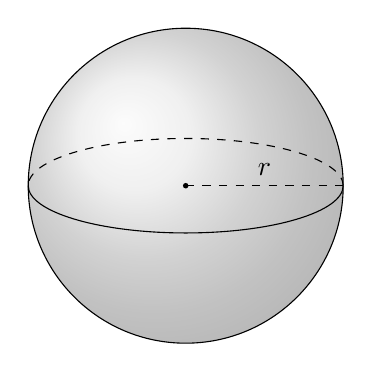
\begin{tikzpicture}
      \shade[ball color = gray!40, opacity = 0.4] (0,0) circle (2cm);
      \draw (0,0) circle (2cm);
      \draw (-2,0) arc (180:360:2 and 0.6);
      \draw[dashed] (2,0) arc (0:180:2 and 0.6);
      \fill[fill=black] (0,0) circle (1pt);
      \draw[dashed] (0,0 ) -- node[above]{$r$} (2,0);
    \end{tikzpicture}
    }
    \only<2>{
        \begin{figure}
            \centering
            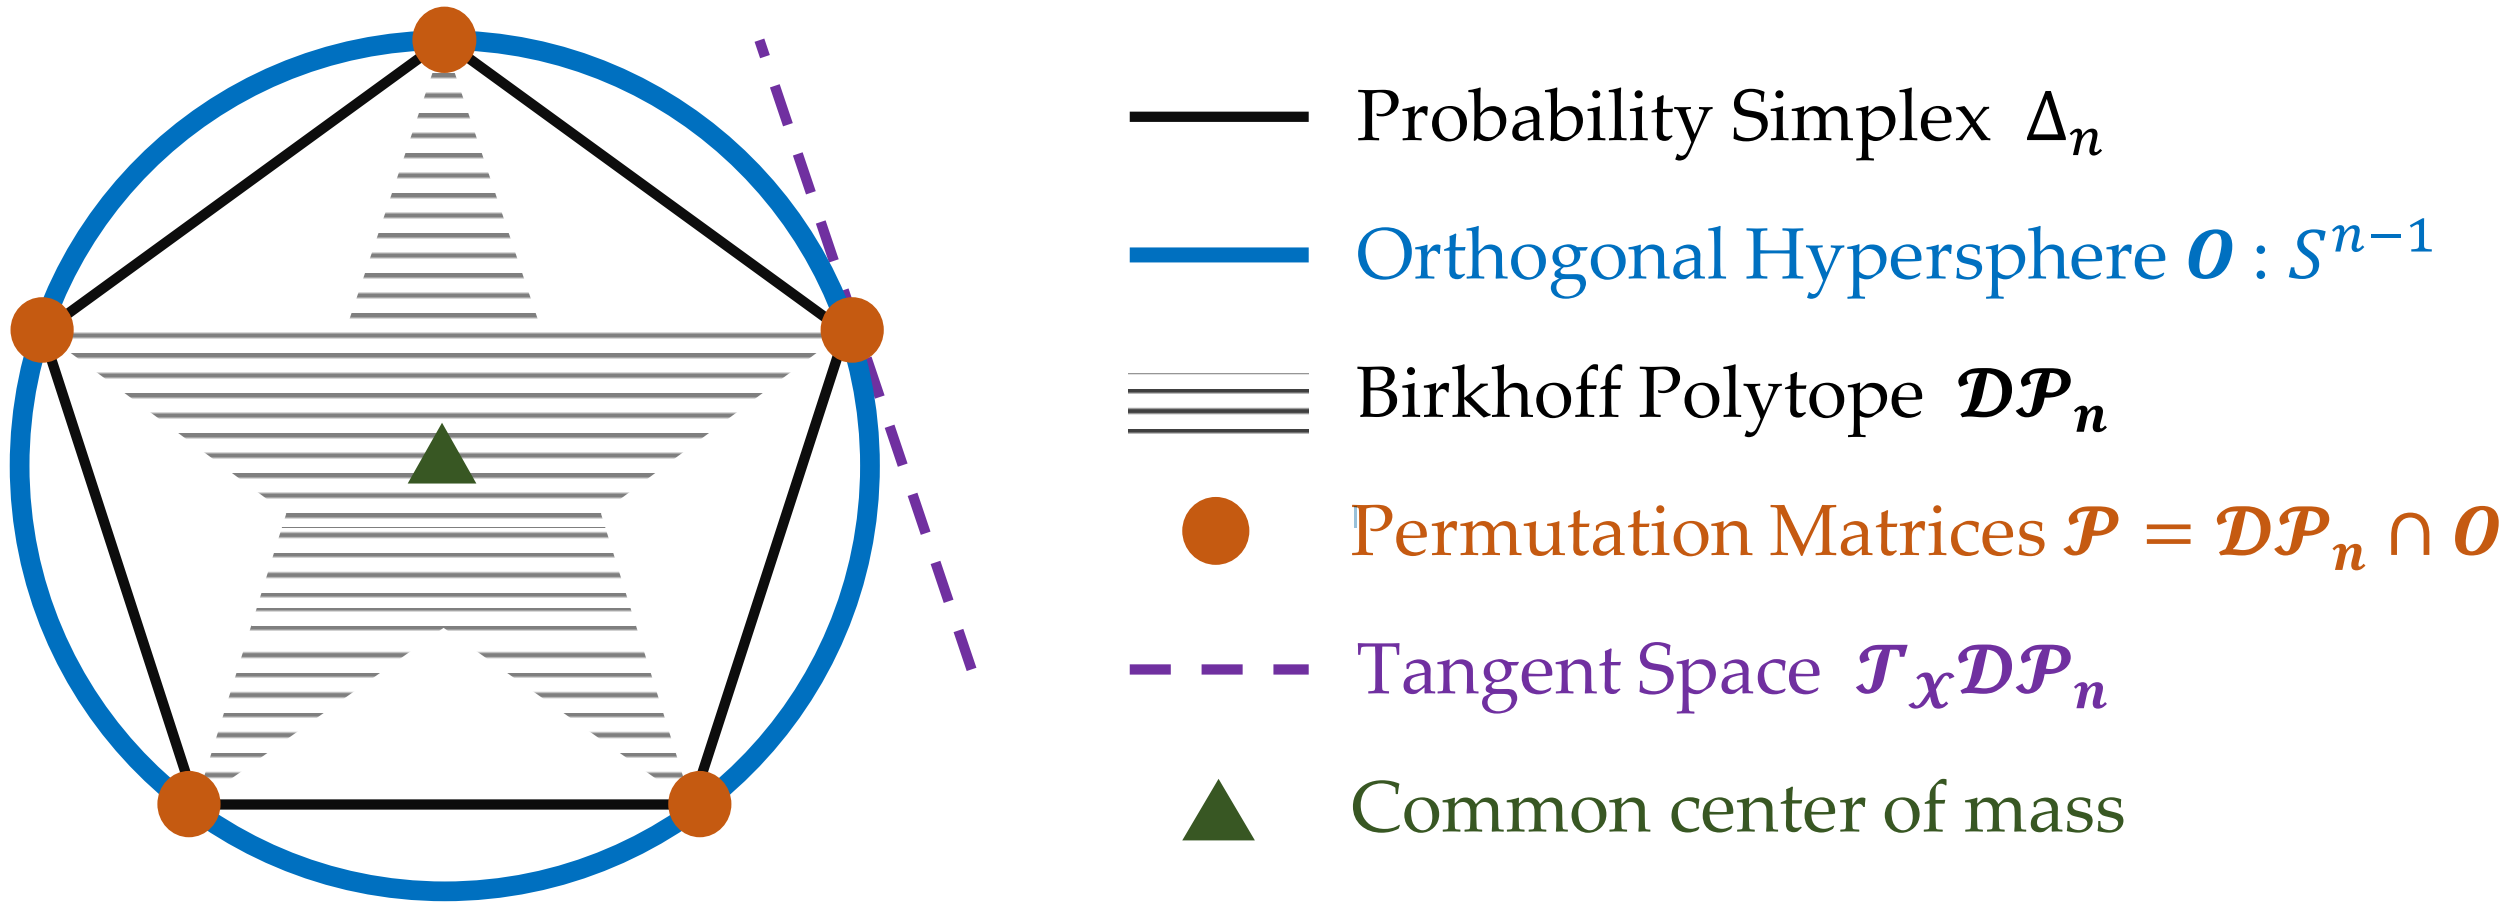
\includegraphics[width=\linewidth]{img/birkhoff.png}
            \caption{\url{https://arxiv.org/abs/1904.05814}}
            \label{fig:my_label}
        \end{figure}
        
    }
    \only<3>{
        \begin{figure}
            \centering
            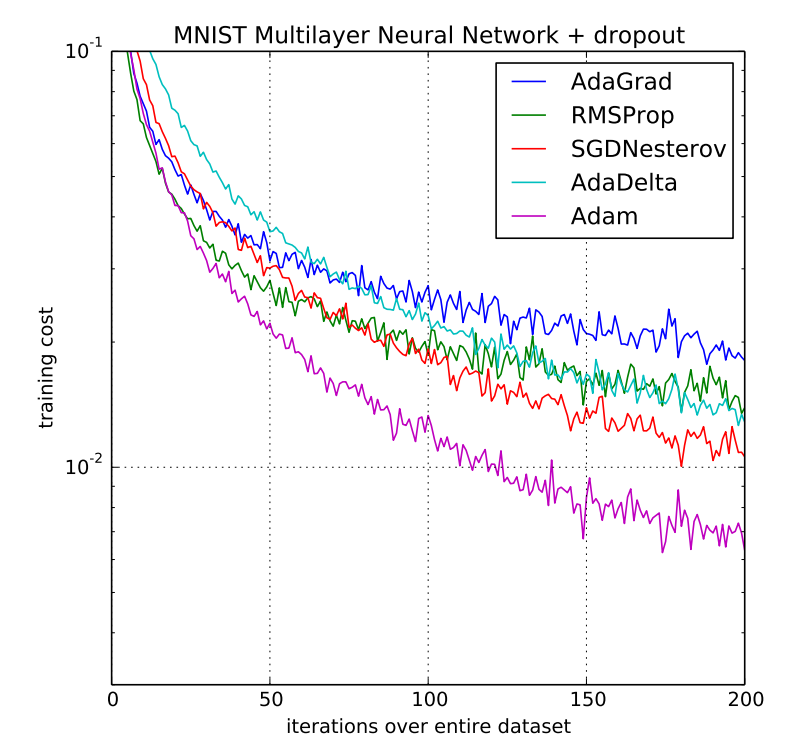
\includegraphics[width=0.8\linewidth]{img/adam_mnist.png}
            \caption{\url{https://arxiv.org/abs/1412.6980}}
            \label{fig:my_label}
        \end{figure}
    }
    \only<4>{
        \begin{figure}
            \centering
            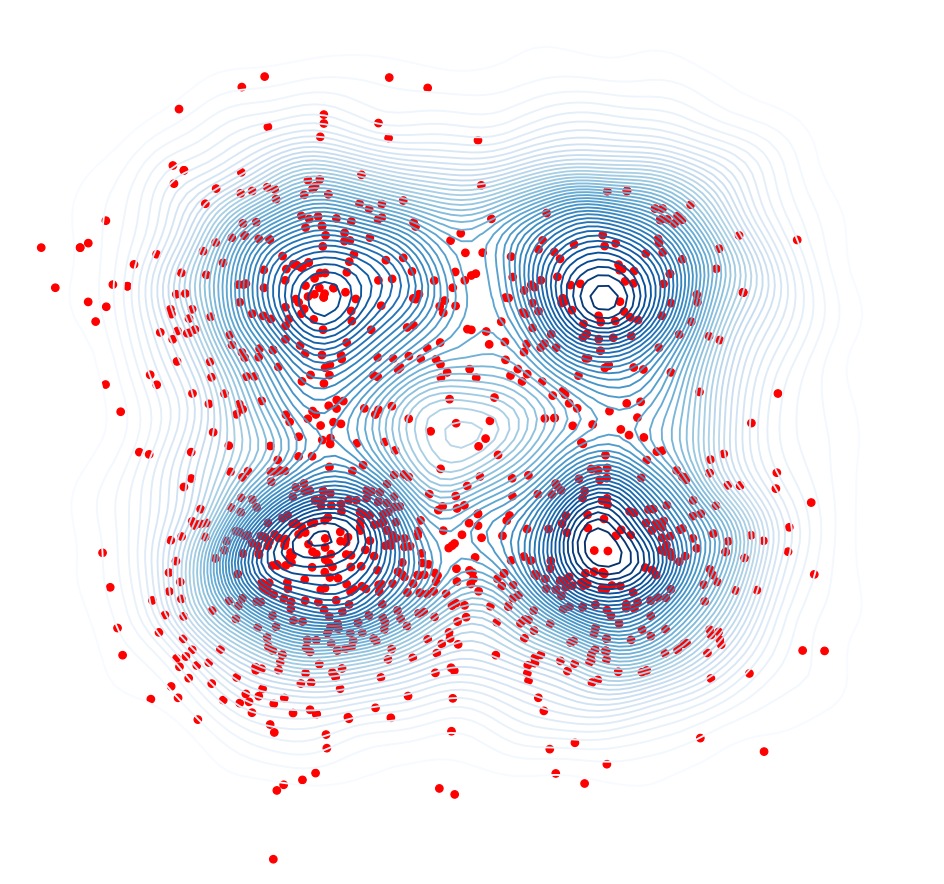
\includegraphics[width=0.8\linewidth]{img/hmc_samples.png}
            \caption{\url{https://arxiv.org/abs/1901.08045}}
            \label{fig:my_label}
        \end{figure}
    }
    \end{column}
    \end{columns}
\end{frame}
\subsection{Alternative Approaches}
\begin{frame}{What else?}
    \begin{columns}
    \begin{column}{0.5\linewidth}
    \begin{itemize}
    \visible<1->{
    \item Reparametrization
    \begin{itemize}
        \item Adaptive terms make sense
        \item HMC is possible
        \item This might be a good idea
    \end{itemize}
    }
    \visible<2>{
    \item Projection
    \begin{itemize}
        \item Adaptive terms do not really make sense
        \item Projection may be hard differentiable (iterative)
    \end{itemize}
    }
    \end{itemize}
    \end{column}
    \begin{column}{0.5\linewidth}
    \begin{tikzpicture}
      \draw (0,0) circle (2cm);
      \fill[fill=black] (0,0) circle (1pt);
      \draw[dashed] (0,0 ) -- node[above]{$v/\|v\|$} (2,0);
      \draw[dashed] (2,0 ) -- node[right,above]{$v$} (3,0);
      \fill[fill=black] (2,0) circle (1pt);
      \fill[fill=black] (3,0) circle (1pt);
    \end{tikzpicture}
    \end{column}
    \end{columns}
\end{frame}
\section{SGD Review}
\begin{frame}{Riemannian AMS grad}
\vspace{-0.5em}
    \begin{figure}
\begin{subfigure}{.45\textwidth}
\centering
\begin{algorithmic}
    \Require $x_1\in\mathcal{X}$, $\lbrace\alpha_t\rbrace_{t=1}^T$, $\lbrace\beta_{1t}\rbrace_{t=1}^T$, $\beta_2$\\
    Set $m_0=0$, $v_0=0$ and $\hat{v}_0=0$
    \For{$t=1$ to $T$} (for all $1\leq i\leq n$)
    \State $\alert<2,7>{g_t=\mathrm{grad} f_t(x_t)}$
    \State $\alert<3,8>{m_t^i=\beta_{1t}m_{t-1}^i+(1-\beta_{1t}) g_t^i}$
    \State $\alert<4,9>{v_t^i=\beta_2 v_{t-1}^i + (1-\beta_2)(g_t^{i})^2}$
    \State $\alert<4,9>{\hat{v}_t^i=\max\{\hat{v}_{t-1}^i,v_t^i\}}$
    \State $\alert<5,10>{x_{t+1}^i=x_{t}^i-\alpha_t m_t^i/\sqrt{\hat{v}_t^i}}$\\
    \visible<8->{\alert<8>{\Comment{no vector transport}}\\}
    \textbf{end\ for}
    \EndFor\\
\end{algorithmic}
    \caption{\textsc{Amsgrad} in $\mathbb{R}^n$.}\label{alg:alg-2}
\end{subfigure}
\hfill
\visible<6->{
\begin{subfigure}{.45\textwidth}
\centering
\begin{algorithmic}
    \Require $x_1\in\mathcal{X}$, $\lbrace\alpha_t\rbrace_{t=1}^T$, $\lbrace\beta_{1t}\rbrace_{t=1}^T$, $\beta_2$\\
    Set $m_0=0$, $\tau_0=0$, $v_0=0$ and $\hat{v}_0=0$
    \For{$t=1$ to $T$} (for all $1\leq i\leq n$)
    \State $\alert<7>{g_t=\mathrm{rgrad} f_t(x_t)}$ 
    \State $\alert<8>{m_t^i=\beta_{1t}\tau_{t-1}^i+(1-\beta_{1t}) g_t^i}$
    \State $\alert<9>{v_t^i=\beta_2 v_{t-1}^i + (1-\beta_2)\Vert g_t^{i}\Vert_{x_t^i}^2}$
    \State $\alert<9>{\hat{v}_t^i=\max\{\hat{v}_{t-1}^i,v_t^i\}}$
    \State $\alert<10>{x_{t+1}^i=\exp^i_{x_{t}^i}(-\alpha_t m_t^i/\sqrt{\hat{v}_t^i})}$
    \State $\alert<8>{\tau_t^i=P^i_{x_t^i\to x_{t+1}^i}(m_t^i)}$\\
    \textbf{end\ for}
    \EndFor\\
\end{algorithmic}
    \caption{\textsc{Ramsgrad} in $\mathcal{M}_1\times\cdots\times\mathcal{M}_n$.}
    \label{alg:alg-1}
\end{subfigure}
}
\end{figure}
Comment: %
\only<2>{we need gradients, in \texttt{pytorch} it would be \texttt{loss.backward()}}%
\only<3>{keep track of momentum at each iteration}%
\only<4>{update adaptive terms using second moments of the gradient}%
\only<5>{sure we make final gradient step}%
\only<6>{what is the difference for Riemannian case?}%
\only<7>{gradient stays \textit{almost} the same, \texttt{loss.backward()} and correction}%
\only<8>{momentum update requires new operation, \textit{``vector transport''} $P^i_{x_t^i\to x_{t+1}^i}$}%
\only<9>{adaptive term depends on the current point via$\Vert g_t^{i}\Vert_{x_t^i}^2$}%
\only<10>{there is no addition between vectors and points}
\end{frame}
\begin{frame}{Blank Spots}
\begin{columns}
\begin{column}{0.5\linewidth}
\begin{enumerate}
    \item<+-> How to properly work with gradients?
    \item<+-> Why some computations depend on the point of application?
    \item<+-> How to work with momentums?
    \item<+-> How to make the final update?
\end{enumerate}
\visible<+->{
    \begin{block}{}
    We will review all this in the next section
    \end{block}
}
\end{column}
\begin{column}{0.5\linewidth}
\begin{figure}
    \centering
    
\includegraphics[width=0.8\linewidth]{img/thinkingface.png}
\end{figure}
\end{column}
\end{columns}
\end{frame}
\section{Differential Geometry}
\subsection{Manifold}
\begin{frame}{What is Manifold?}
\begin{columns}
\begin{column}{0.5\linewidth}
The best example I know is actually Sphere! 
\visible<2->{
\begin{block}{}
A curious researcher (a kid) may ask questions
\end{block}
\begin{enumerate}
    \item<2-> Is it really a sphere or anything else?
    \item<3-> What makes a sphere be a sphere?
    \item<4> How to represent a point on earth?
\end{enumerate}
}
\end{column}
\begin{column}{0.5\linewidth}
\only<1>{
\begin{figure}
    \centering
    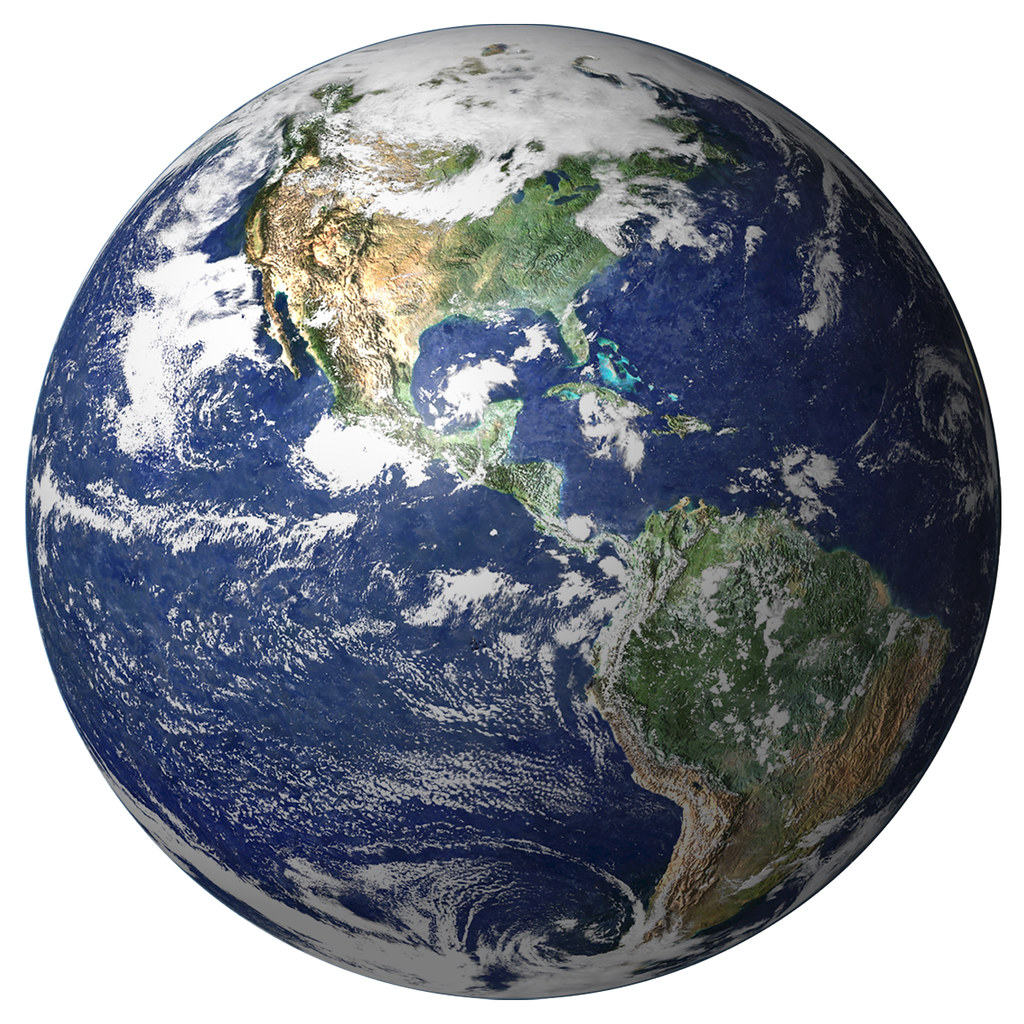
\includegraphics[width=0.8\linewidth]{img/earth.jpg}
    \caption*{Looks like a sphere}
\end{figure}
}%
\only<2>{
\begin{figure}
    \centering
    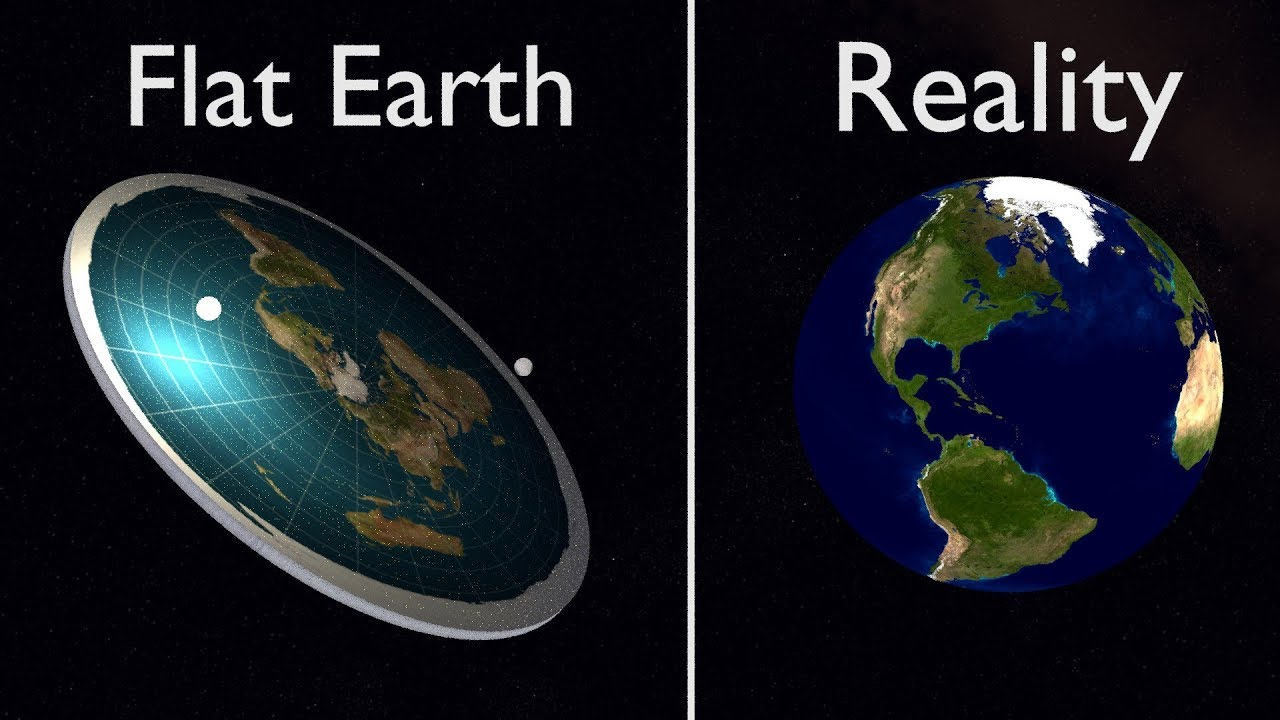
\includegraphics[width=\linewidth]{img/flatearth.jpg}
    \caption*{Or simulation?}
\end{figure}
}%
\only<3>{
\begin{figure}
\centering
\begin{subfigure}{0.5\linewidth}
\centering
    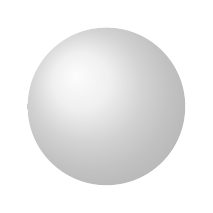
\begin{tikzpicture}
      \shade[ball color = gray!40, opacity = 0.4] (0,0) circle (1cm);
    \end{tikzpicture}
    \caption*{sphere}
\end{subfigure}%
\begin{subfigure}{0.5\linewidth}
\centering
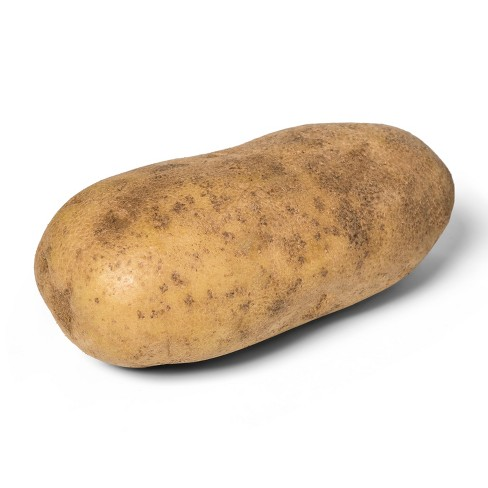
\includegraphics[width=\linewidth]{img/potato.jpeg}
\caption*{also a sphere}
\end{subfigure}
\caption*{Topology joke}
\end{figure}
}%
\only<4>{
\centering
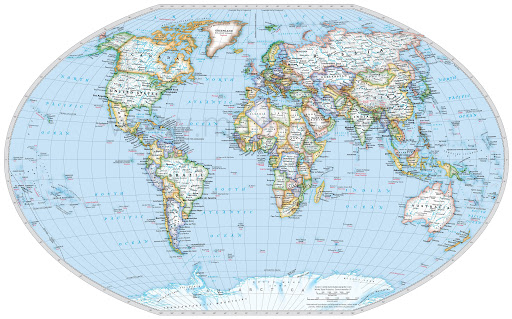
\includegraphics[height=2cm]{img/map1.jpg}
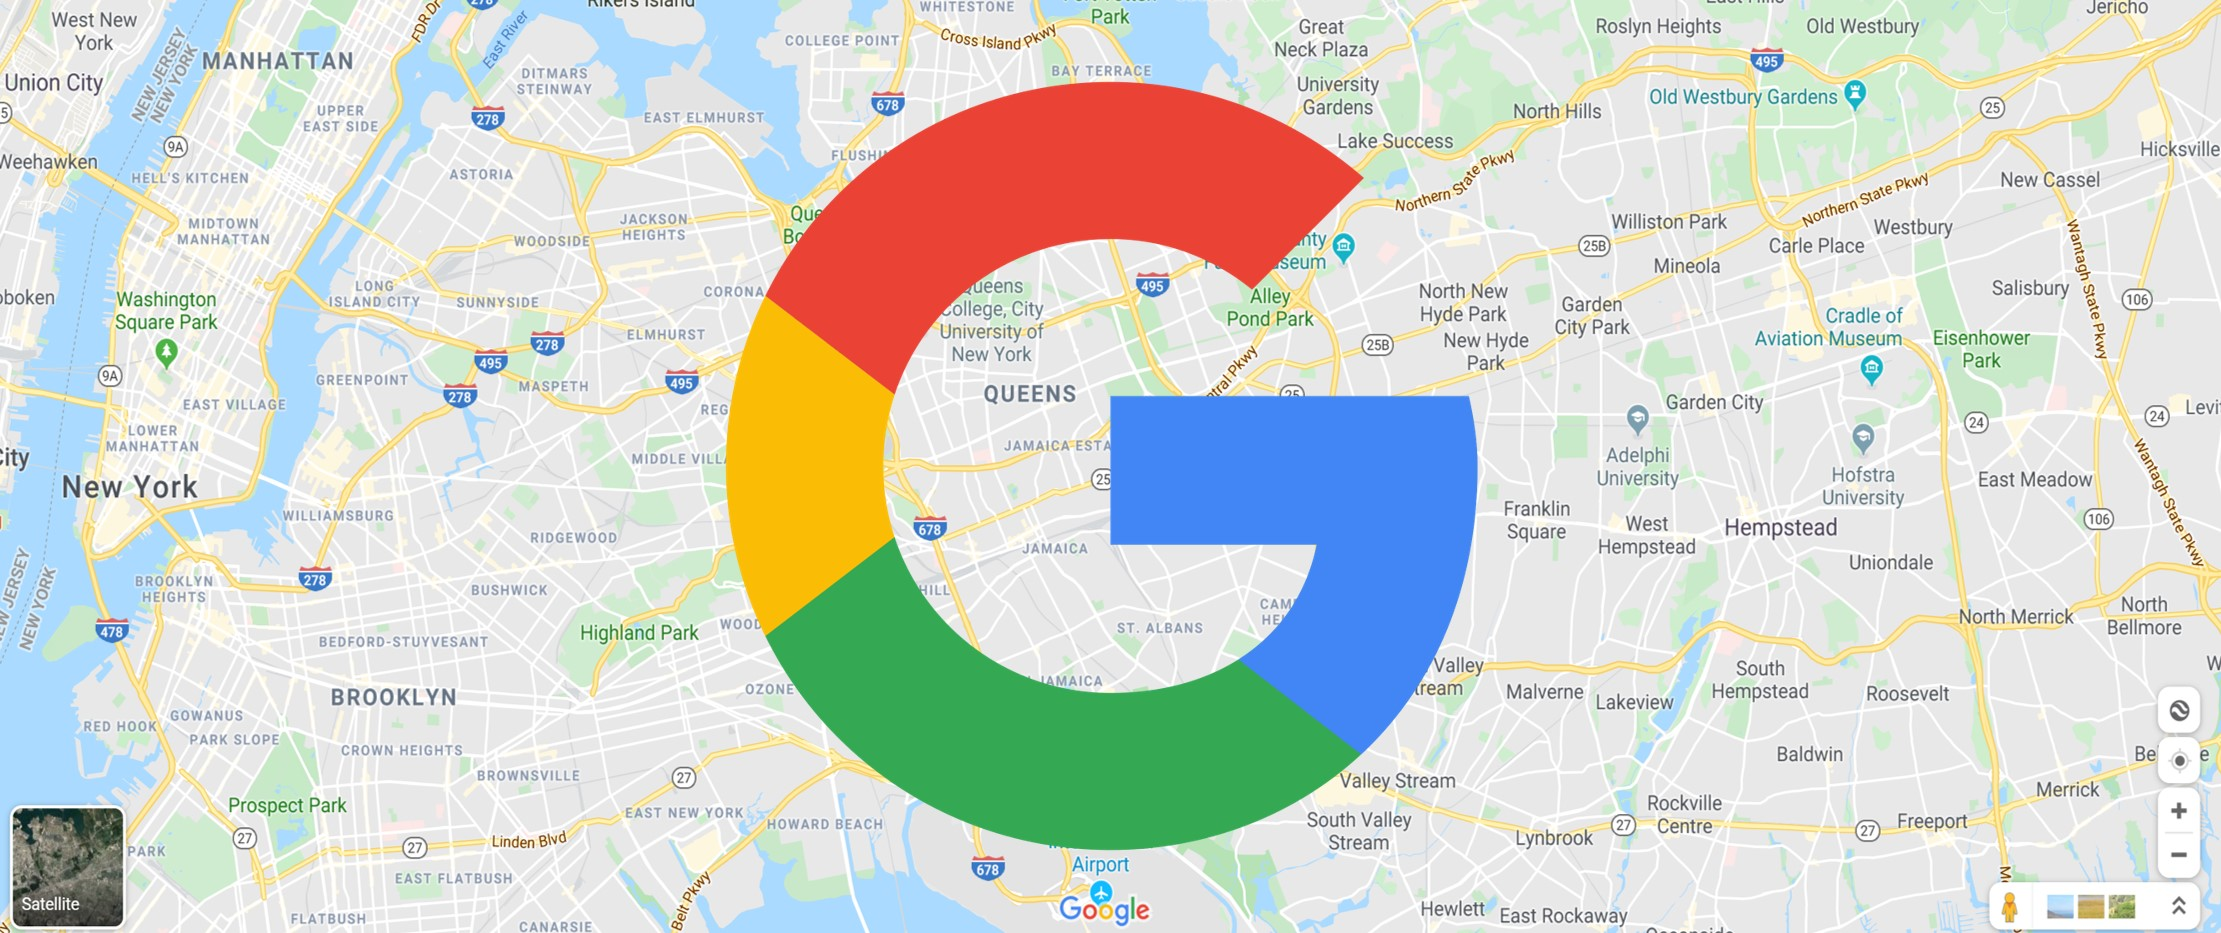
\includegraphics[height=2cm]{img/map2.jpg}\\
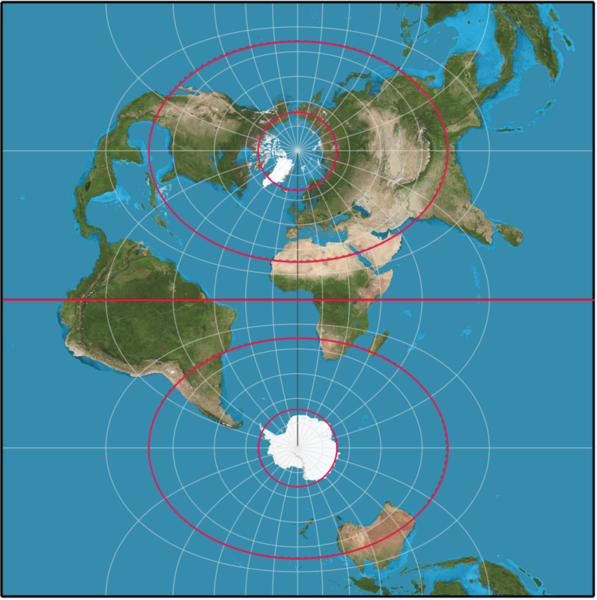
\includegraphics[height=2cm]{img/map3.png}
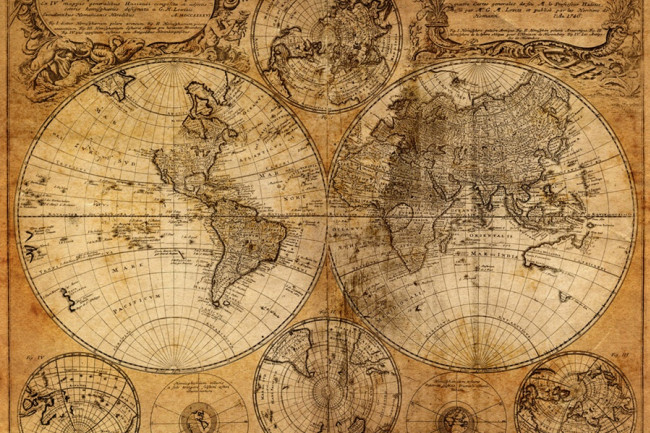
\includegraphics[height=2cm]{img/map4.jpg}\\
}
\end{column}
\end{columns}
\end{frame}
\begin{frame}{Earth is Math}
\begin{columns}
\begin{column}{0.5\linewidth}
\begin{itemize}
    \item ``Sphereness'' is an intrinsic property, we can touch it, but how?
\end{itemize}
\begin{block}{enough?}
\begin{equation*}
    \left\{\|x\| = 1\::\: x \in \sR \right\} 
\end{equation*}
\end{block}
\visible<2>{
\begin{alertblock}{}
no
\end{alertblock}
}
\end{column}
\begin{column}{0.5\linewidth}
\begin{figure}
    \centering
    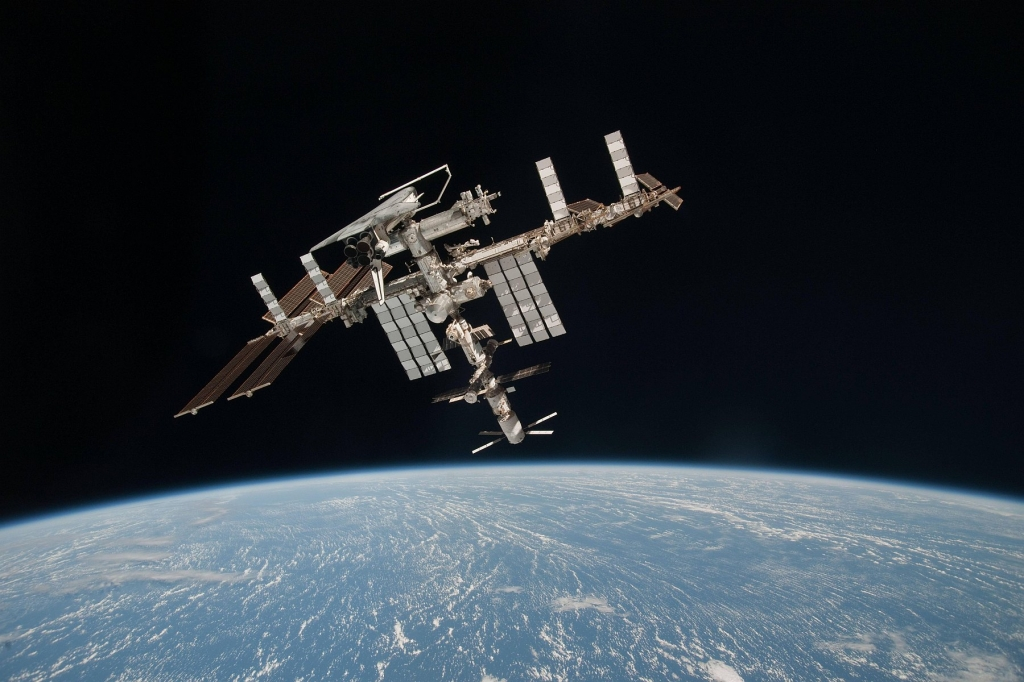
\includegraphics[width=0.8\linewidth]{img/sputnik.jpg}
    \caption*{It's all nature, and we can observe it with experience}
\end{figure}
\end{column}
\end{columns}
\end{frame}
\begin{frame}{Earth is more Math}
\begin{columns}
\begin{column}{0.5\linewidth}
We can represent sphere in many ways:
\begin{block}{Constraints}
\begin{equation*}
    \left\{x : x \in \sR, \|x\| = 1  \right\} 
\end{equation*}
\end{block}
\begin{block}{Angles}
\begin{equation*}
    \left\{(\theta, \phi) : \theta\in (0, \pi), \phi\in (-\pi, \pi)\right\}
\end{equation*}
Note: some points are not covered but this is not a concern
\end{block}
\visible<2>{
\begin{alertblock}{Need more structure}
    We need tangent space defined to explain earth is not a potato
\end{alertblock}
}
\end{column}
\begin{column}{0.5\linewidth}
\begin{figure}
\centering
    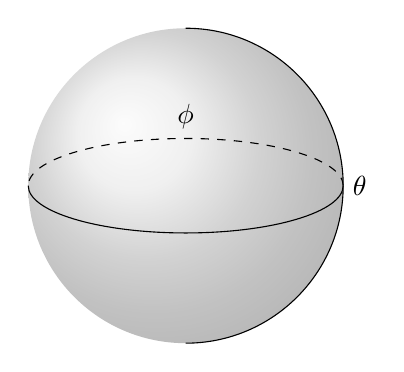
\begin{tikzpicture}
      \shade[ball color = gray!40, opacity = 0.4] (0,0) circle (2cm);
      \draw (0,-2) arc (-90:90:2) node[midway,right]{$\theta$};
      \draw (-2,0) arc (180:360:2 and 0.6);
      \draw[dashed] (2,0) arc (0:180:2 and 0.6) node[midway,above]{$\phi$};
    \end{tikzpicture}
\end{figure}%
\end{column}
\end{columns}
\end{frame}
\subsection{Tangent Space}
\begin{frame}{Velocity}
\begin{columns}
\begin{column}{0.5\linewidth}
You can think about points on the manifold like about the picture above.
\begin{itemize}
    \item<1-> GPS gives you \textit{coordinates} on the manifold $(\phi, \theta)$ for $p\in \gM$
    \item<2-> Riding a car you have \textit{velocity} $(\dot\phi, \dot\theta) \in T_p\gM$ \textit{at that point}
    \item<3-> A tuple $([\phi, \theta]; [\dot\phi, \dot\theta])$ is from tangent boundle $T\gM$
\end{itemize}
\begin{block}{Notation}
\begin{itemize}
    \item<1-> $\gM$ -- Manifold
    \item<2-> $T_p\gM$ -- tangent space at point $p$
    \item<3-> $T\gM$ -- tangent boundle
\end{itemize}
\end{block}
\end{column}
\begin{column}{0.5\linewidth}
\begin{figure}
    \centering
    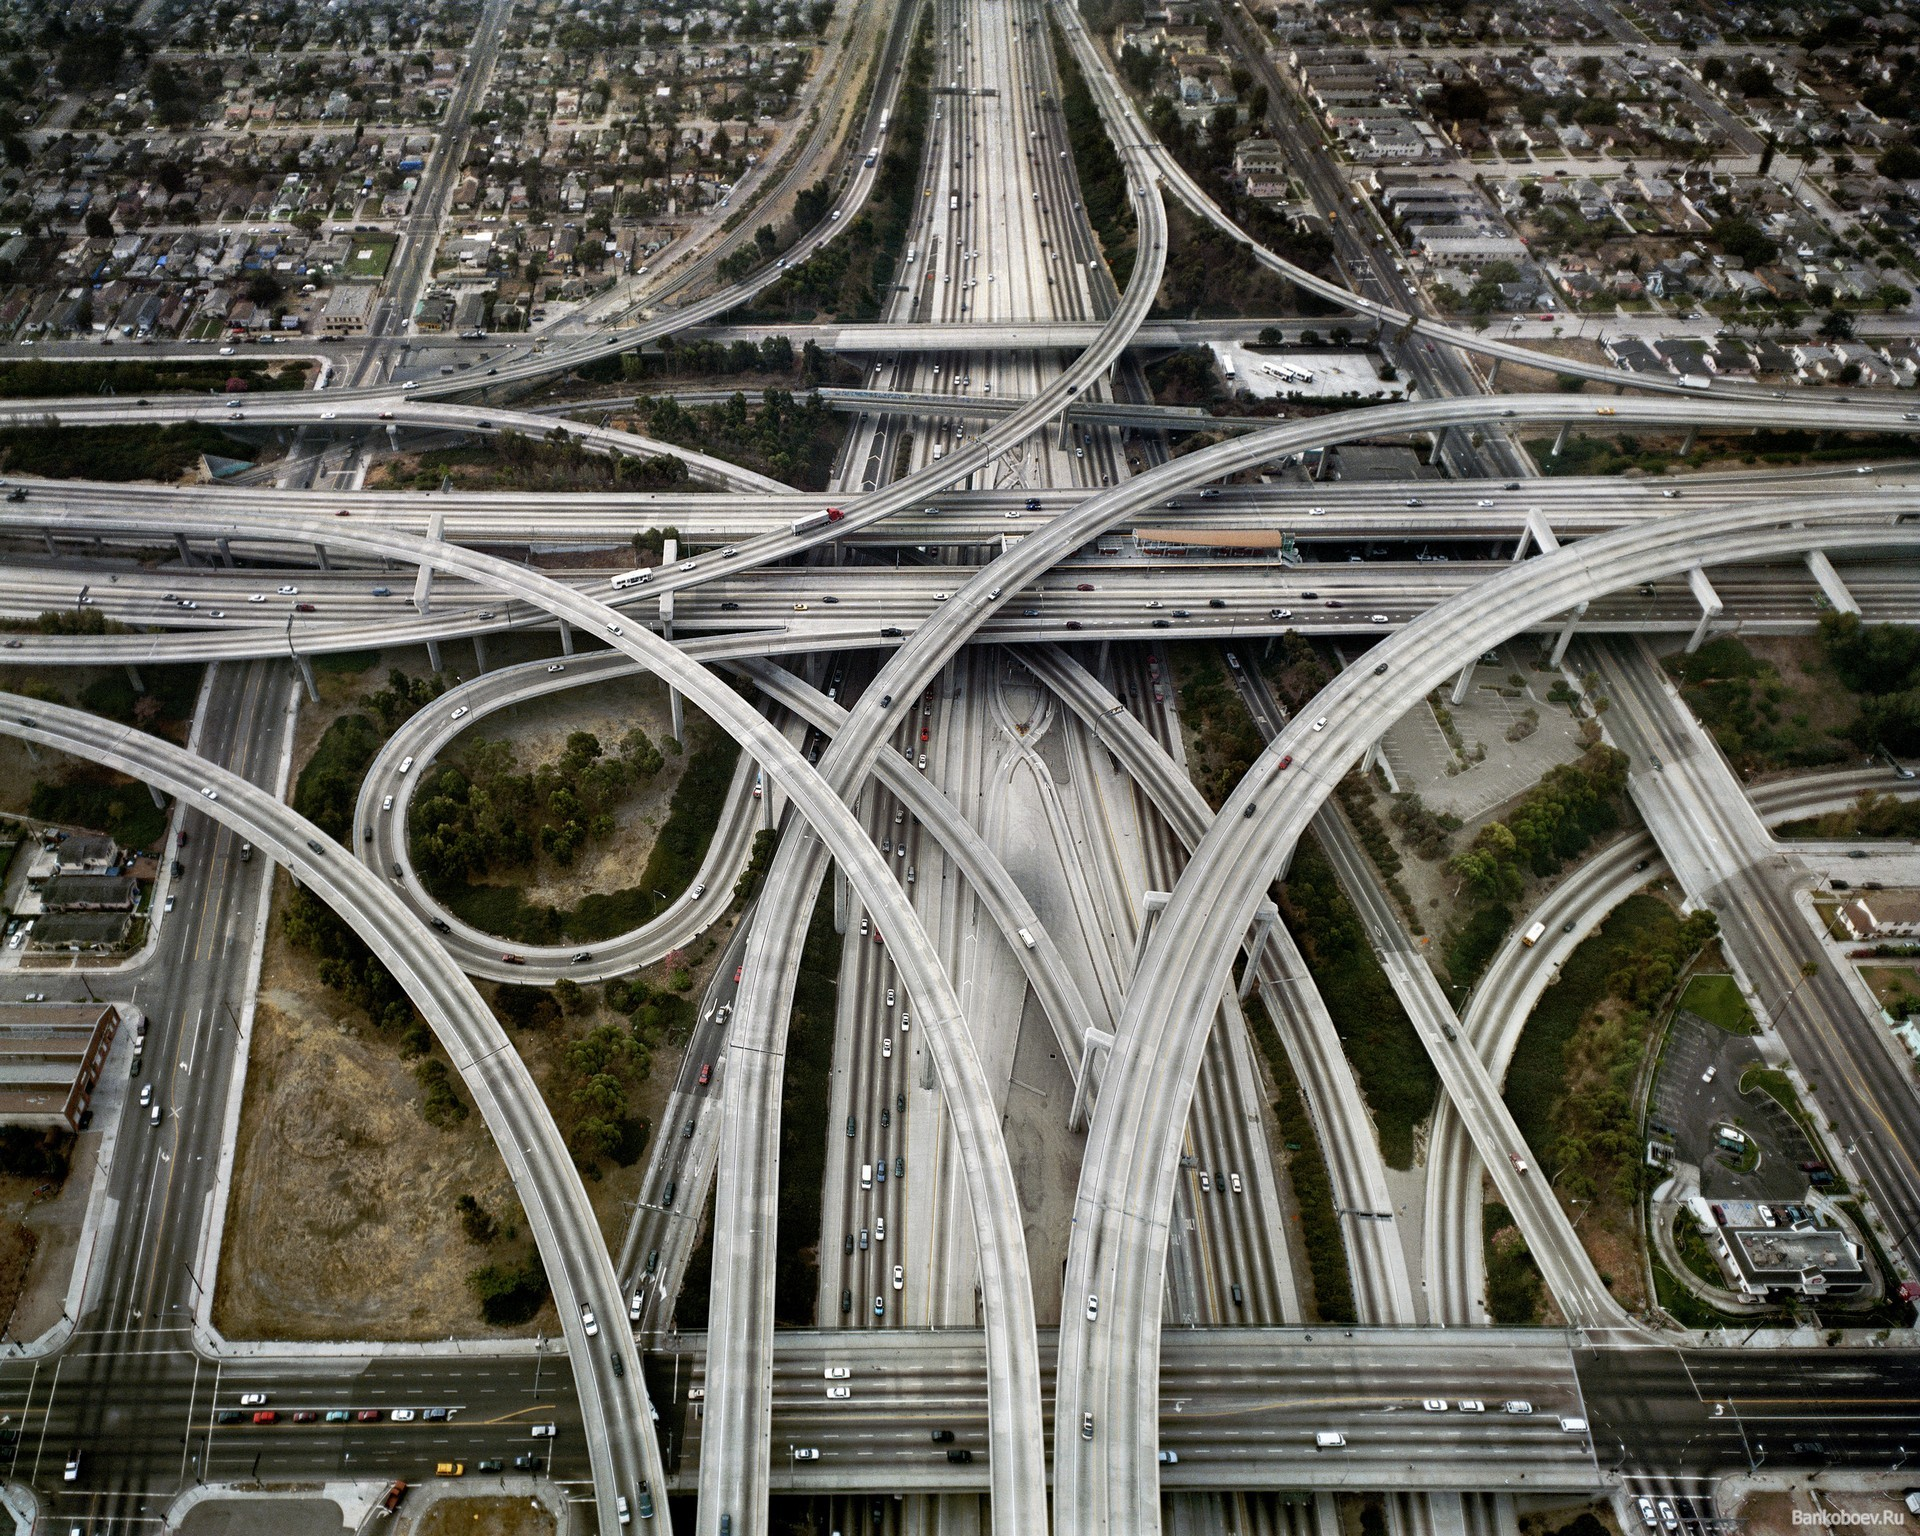
\includegraphics[width=\linewidth]{img/lots-of-roads.jpg}
    \caption*{$(33.9283703,-118.2808926)\in \gM$ on Earth}
\end{figure}
\end{column}
\end{columns}
\end{frame}
\begin{frame}{Tangent Boundle}
\begin{columns}
\begin{column}{0.7\linewidth}
So the tangent boundle $T\gM$ is a disjoint union of all points $p\in\gM$ and velocities $v\in T_p\gM$ at that point
\begin{equation*}
    T\gM = \left\{(p, v) : p\in \gM, v\in T_p\gM \right\}
\end{equation*}
\begin{block}{Note}
    We can go back and forth between $\gM$ and  $T\gM$ using
    \begin{itemize}
        \item Vector field, $V : \gM\to T\gM$
        \item Canonical projection, $\pi: (p, v) \mapsto p$
    \end{itemize}
\end{block}
\end{column}
\begin{column}{0.3\linewidth}
\begin{figure}
    \centering
    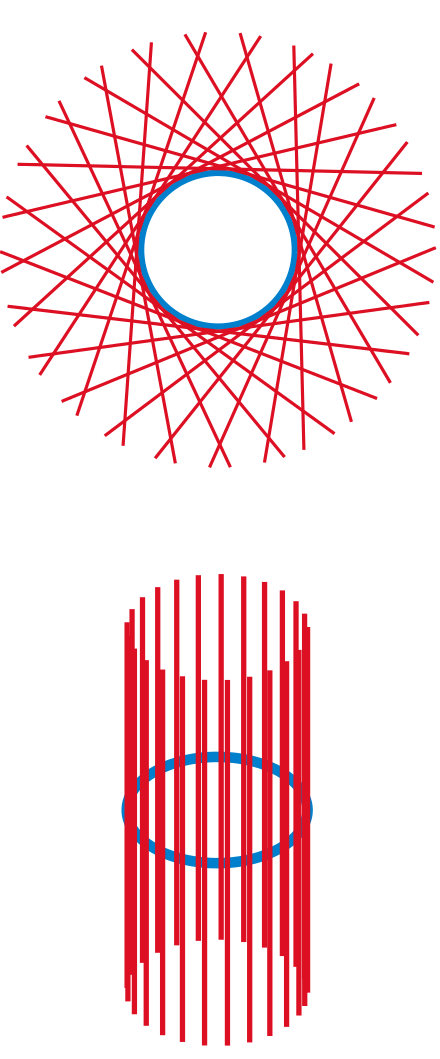
\includegraphics[width=0.5\linewidth]{img/tangent_boundle_wiki.png}
    \caption*{Source: \href{https://en.wikipedia.org/wiki/Tangent_bundle}{wiki}}
    \label{fig:my_label}
\end{figure}
\end{column}
\end{columns}
\end{frame}
\subsection{Curves}
\begin{frame}{Curve}
\begin{columns}
\begin{column}{0.5\linewidth}
Travelling a car you draw a curve on the Earth manifold.

\begin{block}{Definition}
\begin{equation}
    \gamma: \sR \to \gM
\end{equation}
\end{block}
In math it maps (0, 1) interval to the Manifold. 
In reality you can think of mapping time to GPS location in the car.

For the curve you have speed, 
\end{column}

\begin{column}{0.5\linewidth}
\begin{figure}
    \centering
    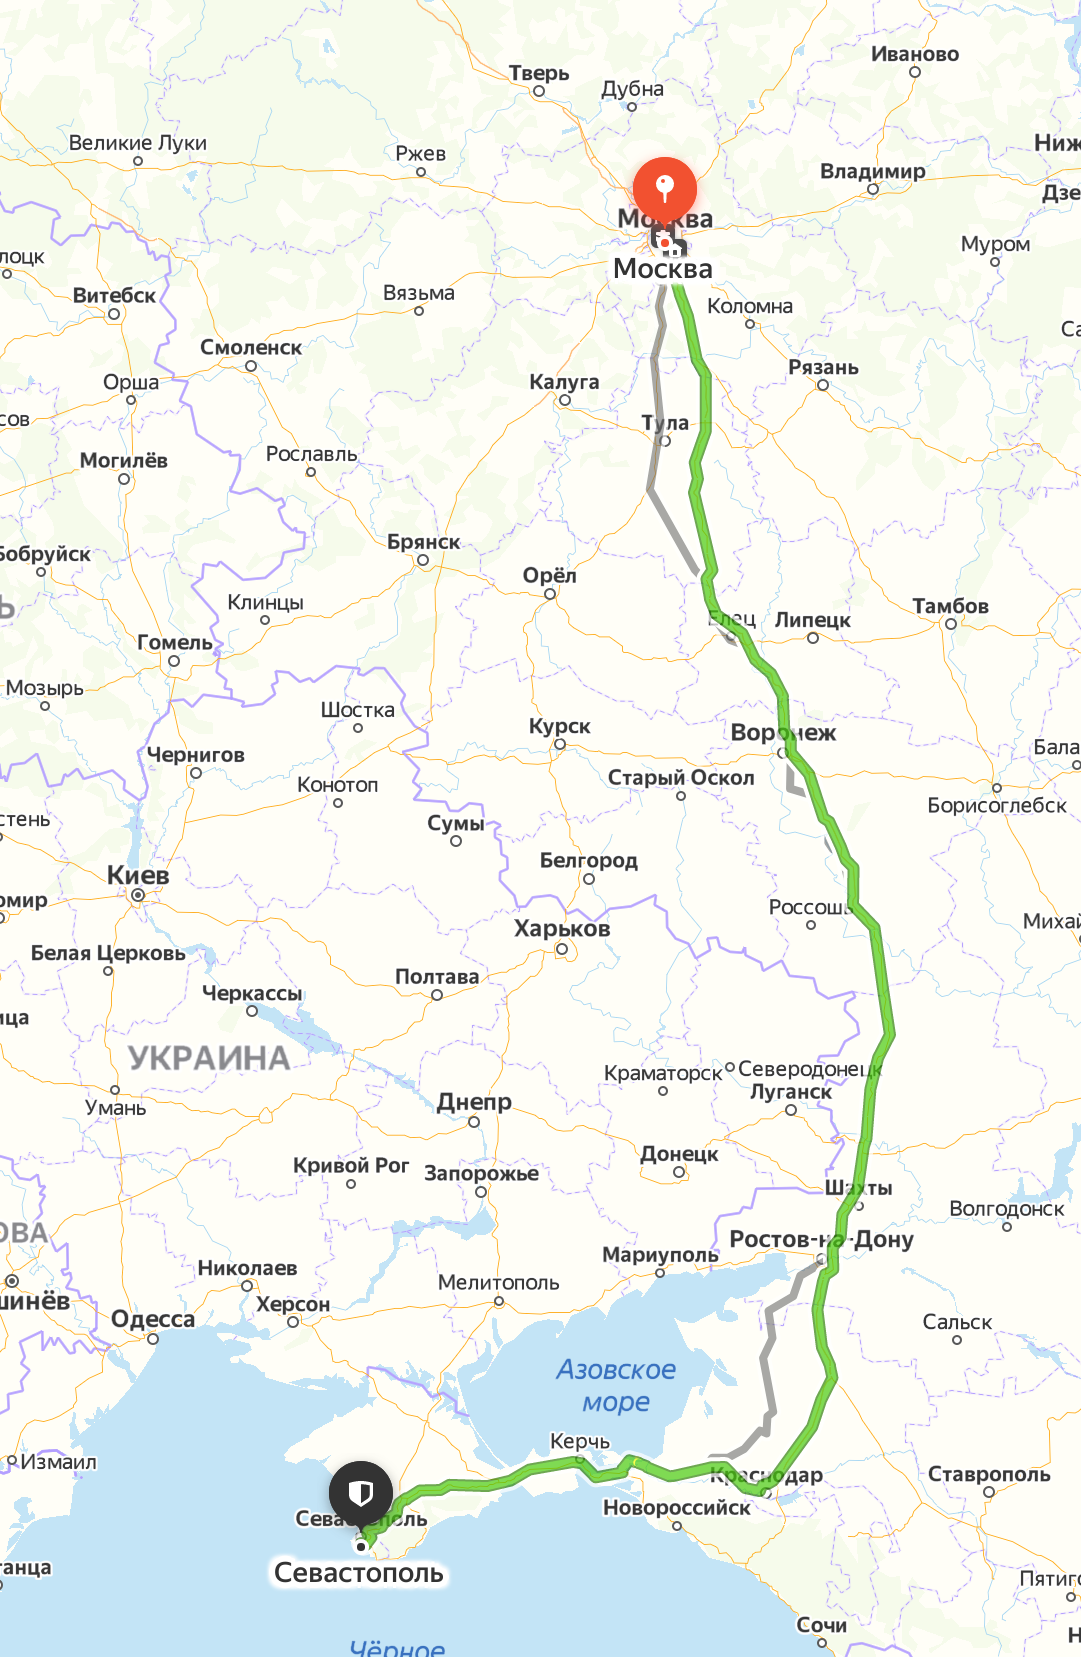
\includegraphics[height=6.4cm]{img/route.png}
\end{figure}
\end{column}
\end{columns}
\end{frame}
\subsection{Inner Product}
\subsection{Vector Transport}
\section{Filling Blank Spots}
\subsection{Computing Gradient}
\subsection{Computing Adaptive Term}
\subsection{Updating Momentum}
\section{Practical Implementation}
\end{document}
